\documentclass[main]{subfiles}

\begin{document}

\chapter{Software}
\label{chap:Software}

El objetivo de esta sección es realizar una breve introducción sobre cómo utilizar la impementaci\'on en software del vuelo autónomo del cuadricóptero. Para entender en detalle qué hace cada función, referirse a los comentarios en el código fuente, disponible en el repositorio git, en la carpeta \verb+src/+. Todas las referencias a archivos son respecto a la raíz del repositorio. Los programas están pensados para compilarse y ejecutarse en un entorno \emph{Linux}.\\

En el anexo \ref{chap:anexo-codigo} se explica como compilar y configurar las partes involucradas.

\section{Esquema general}
\label{sec:software:esquema-general}

\begin{wrapfigure}{r}{0.6\textwidth}
\vspace{-20pt}
\centering
  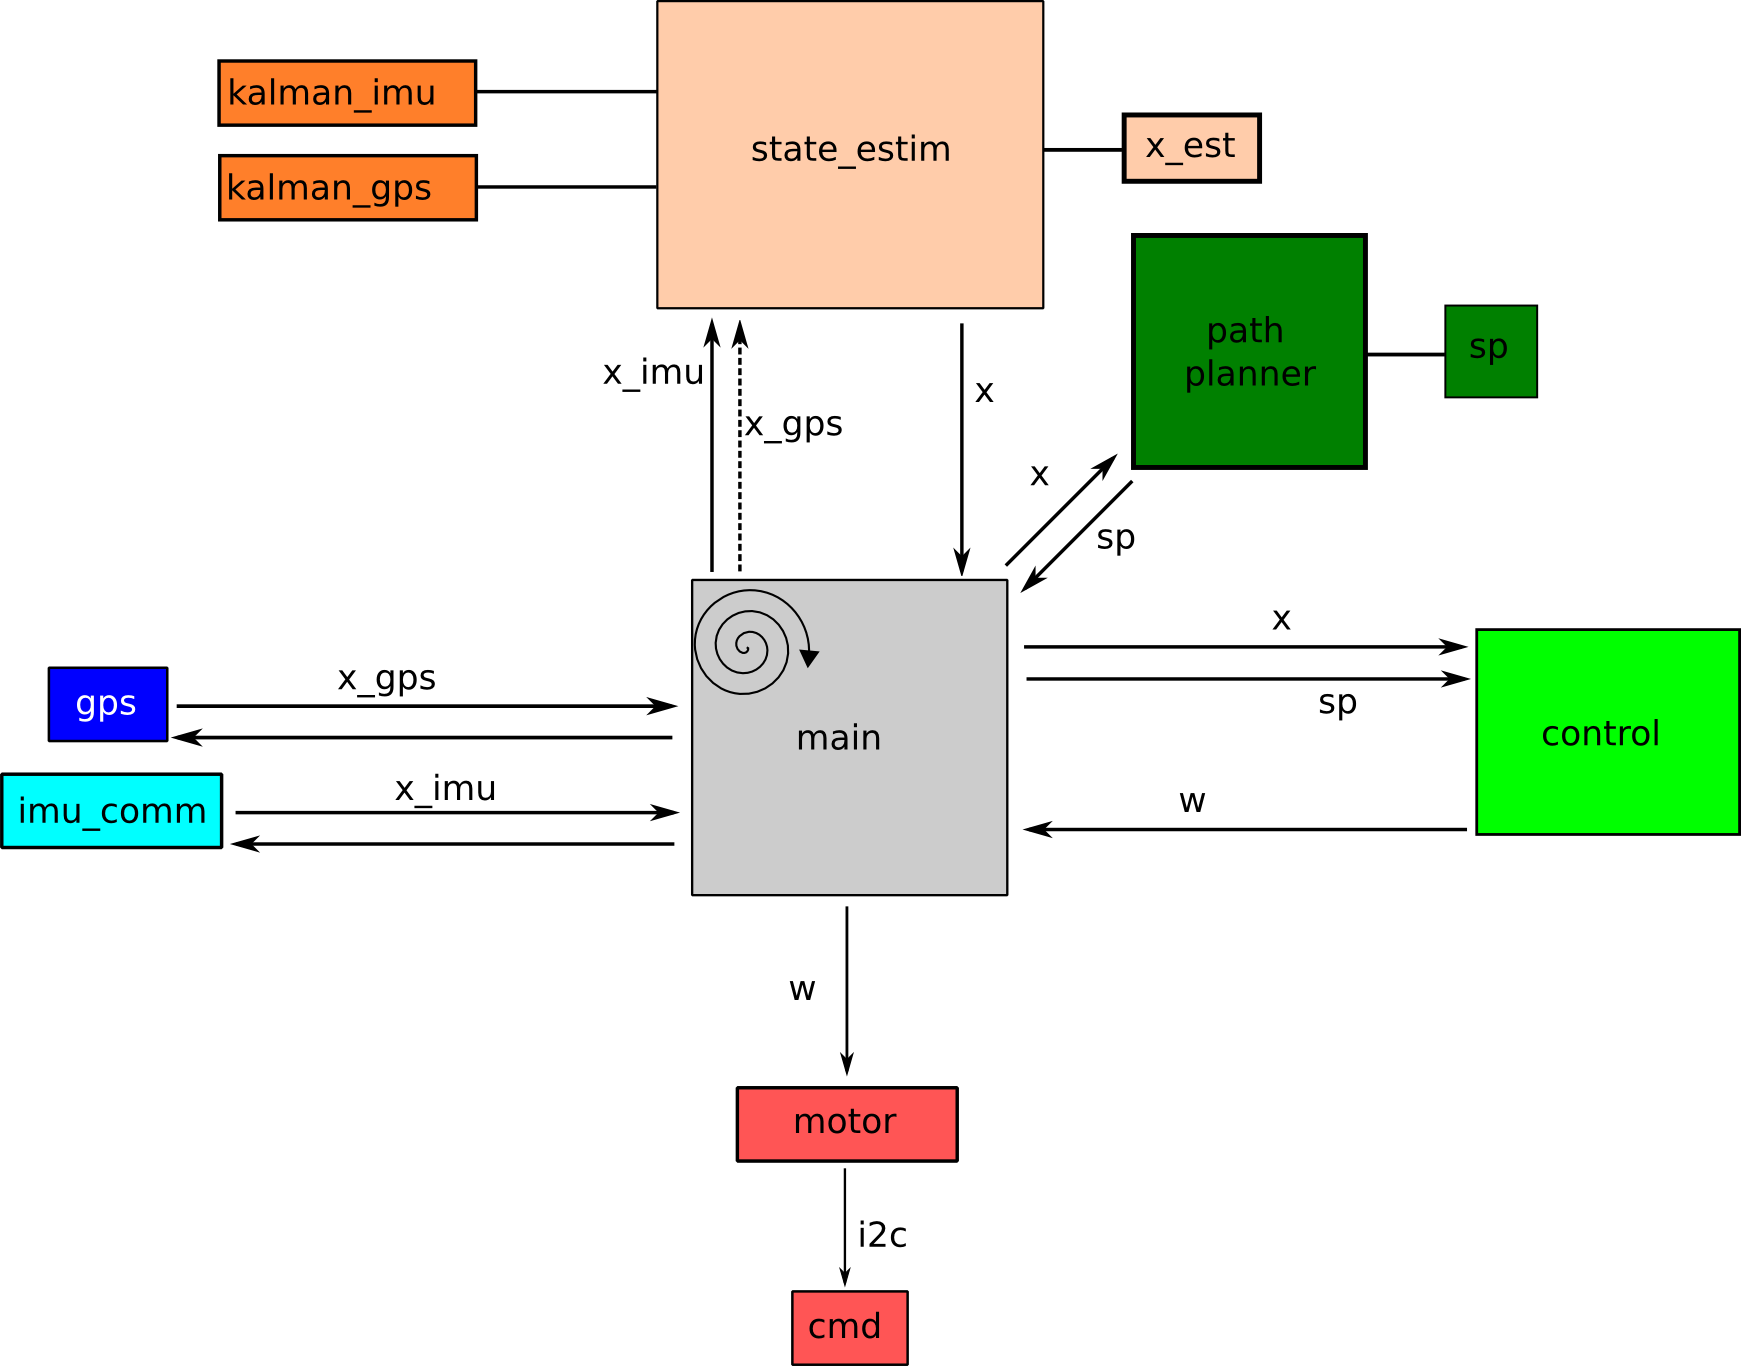
\includegraphics[width=0.5\textwidth]{./pics_codigo/code.png}
\caption{Estructura general del código.}
\vspace{-20pt}
\label{fig:codigo:code.png}
\end{wrapfigure}

El código tiene una estructura modular, está escrito en C, y cada bloque está implementado como una biblioteca. La estructura general del código se resume en la figura \ref{fig:codigo:code.png}. Por claridad no se muestran los bloques intermedios utilizados para intercomunicar las distintas partes.

\section{Inicializaci\'on}
\label{sec:software-init}

Para correr el programa principal (de ahora en más: \textit{main}) deber\'ia bastar con ejecutar el script \verb+src/go.sh+.\\

Durante la inicializaci\'on el \textit{main} debe encontrar lo siguiente:
\begin{itemize}
\item \verb+imu_calib.txt+: Par\'ametros de calibraci\'on, la biblioteca \textit{imu\_comm} los necesita para convertir los datos crudos provenientes de la IMU.
\item \verb+K*.txt+: Matrices de control utilizados en el modo \textit{hover}.
\item \verb+lqr-*.txt+: Par\'ametros del algoritmo \textit{LQR}.
\item IMU: La IMU env\'ia datos a trav\'es de una \textit{UART} que es mapeada por el sistema operativo a un ``archivo'' \verb+/dev/tty*+. El \textit{main} buscar\'a este archivo, o en su defecto un log \verb+imu_raw.txt+ generado por el \textit{main} en una ejecuci\'on previa.
\item GPS: Los datos provenientes del GPS  (\textit{USB}) son mapeados por el sistema operativo a \verb+/dev/ttyUSB*+). No se interactua directamente con este archivo, se utiliza la biblioteca \textit{gps\_comm} para iniciar un cliente que se comunique con el \textit{gpsd}, que es el programa que se encarga de leer y analizar los datos crudos provenientes del GPS. El \textit{gpsd} es iniciado por el script \verb+go.sh+.\newline
Si no se dispone de se\~nal del GPS se puede configurar un modo de prueba en el que se simulan los datos del GPS (a 1Hz) generando ceros, o números al azar dentro de un rango dado.
\item \verb+cmd+: El driver de los motores, encargado exclusivamente de env\'iar continuamente comandos \textit{i2c} a los ESCs con la \'ultima velocidad configurada\footnote{Los motores se apagan si no reciben comandos continuamente.}. Durante pruebas, se puede configurar el driver para que simule la presencia de los motores, o para que lea de la entrada est\'andar. Ver \verb+src/i2c_beagle/README+ por informaci\'on sobre como compilar los distintos modos.\newline
La comunicaci\'on entre el driver y el \textit{main} se realiza mediante la biblioteca \textit{motor}, que a su vez se comunica con el driver mediante colas de kernel (IPC\footnote{\textit{Interprocess Communication}: \url{http://www.cs.cf.ac.uk/Dave/C}.}), utilizando la biblioteca \textit{uquad\_kernel\_msgq}.
\end{itemize}

\section{Loop}
\label{sec:software-loop}

A continuaci\'on se describe un loop normal ejecutado por el \textit{main}, explicando brevemente las funcionalidades de cada una de las bibliotecas involucradas:
\begin{enumerate}

\item \textbf{imu:} La IMU genera datos nuevos cada 10ms. Al comienzo del loop, el \textit{main} revisa si hay datos nuevos, y en caso afirmativo llama a la biblioteca para que los lea. Cuando se completa una trama, los datos crudos se almacenan en una cola circular. Al terminar de recibir una trama, se vuelve al principio del loop para verificar que no hay m\'as nada para leer, en caso de haber m\'as datos entonces el hay que leerlos para evitar atrasarse respecto a la IMU.

\item \textbf{gps:} El GPS genera datos nuevos a una tasa mucho menor que la IMU. Cada vez que se dispone de una muestra nueva en la IMU, el \textit{main} revisa si tambi\'en hay un dato nuevo del GPS, y avanza aunque no se disponga de datos nuevos del GPS.

\item \textbf{kalman:} El filtro de Kalman est\'a implementado en la biblioteca \textit{kalman}. Recibe una estructura de datos generada por \textit{imu\_comm} y otra (opcional) generada por \textit{gps\_comm}. Mantiene una estructura de datos que almacena el estado estimado y las matrices de covarianza.

\item \textbf{path planner:} El m\'odulo generador de rutas est\'a implementado en la biblioteca \textit{path\_planner}. Compara el estado actual con el objetivo, y determina si se completó el objetivo actual\footnote{Solamente se implement\'o el modo \textit{hover}.}. En caso afirmativo, devuelve una bandera que le indicar\'a al m\'odulo de control que debe actualizar la matriz de control para ajustarla a la nueva trayectoria.

\item \textbf{control:} El m\'odulo de control est\'a implementado en la biblioteca \textit{control}. Mantiene una estructura con las matrices del control proporcional e integral (si corresponde). Recibe como argumento el estado estimado y la velocidad actual de los motores, y una estructura generada por \textit{path\_planner}, que indica el estado objetivo y la trayectoria. Devuelve la acci\'on de control a aplicar sobre los motores.

\item \textbf{motor:} Se env\'ia al driver una nueva velocidad deseada.

\end{enumerate}

Por información relativa a bloques, configuración, compilación, ejecución, etc, referirse a:
\begin{quote}
\begin{quote}
\begin{verbatim}
src/README
\end{verbatim}
\end{quote}
\end{quote}

\section{M\'odulo \textit{imu\_comm}}
\label{sec:software:imu-comm}

A continuaci\'on se decriben algunas de las funcionalidades a destacar de la biblioteca \textit{imu\_comm}.

\begin{itemize}
\item \textbf{Calibración:} Se acumulan un conjunto de muestras que después se utilizan para estimar el offset de los giróscopos, y la altura inicial. Estos datos tambi\'en pueden ser utilizados para inicializar el filtro de \textit{Kalman}.\newline
Durante la calibraci\'on, es cr\'itico que el cuadric\'optero no se mueva, ya que en caso de hacerlo las lecturas de los gir\'oscopos ser\'an siempre incorrectas.\newline
La inclinaci\'on afecta la estimaci\'on inicial del offset en los aceler\'ometros, pero en caso de no estar perfectamente horizontal se acomodar\'a luego de unos segundos, no es algo cr\'itico.
\item \textbf{Conversión:} Cargando parámetros de calibración, es posible conviertir datos crudos provenientes de los sensores (cuentas de un ADC) a datos útiles:
  \begin{itemize}
  \item Aceler\'ometro $\rightarrow$ Aceleraciones.
  \item Gir\'oscopo $\rightarrow$ Velocidad angulares.
  \item Aceler\'ometro \verb~+~ Magnet\'ometro  $\rightarrow$ \'Angulos de Euler.
  \item Bar\'ometros $\rightarrow$ Altura y temperatura.
  \end{itemize}

\item \textbf{Filtrado}: Se disponen de funciones que permiten obtener el elemento m\'as nuevo que a\'un no ha sido utilizado, o el resultado de aplicar un filtro FIR\footnote{Los coeficientes del filtro est\'an definidos en \textit{imu\_comm\_init()}.} a los 6 elementos m\'as recientes de la cola. Si por problemas de tiempo el \textit{main} se retrasa, pueden haber datos que nunca sean etiquetados como ``el dato m\'as nuevo'', ya que se leer\'a hasta ponerse al dia. De cualquier forma, ser\'an tomados en cuenta en el filtro.

\item \textbf{Modo \textit{FAKE}:} Seteando \verb+IMU_COMM_FAKE+ a 1, la biblioteca leerá de un log, en lugar de utilizar el puerto serie. Las características fundamentales del modo \textit{FAKE} son:
  \begin{itemize}
  \item Los tiempos no son un problema cr\'itico ya que no correr\'a en tiempo real.
  \item La información en los logs está guardaba en \verb+ascii+ (la IMU trabaja en binario).
  \end{itemize}
\end{itemize}

\section{M\'odulo \textit{kalman}}
\label{sec:software:kalman}

Aparte de implementar el filtro de Kalman descrito en la secci\'on \ref{chap:kalman}, la biblioteca \textit{kalman} se encarga de suavizar la estimaci\'on del \'angulo \textit{theta} dada por los aceler\'ometros y los magnet\'ometros. El ru\'ido presente en los aceler\'ometros, sumado a la mala performance del magnet\'ometro en lugares cerrados\footnote{En los lugares donde se hicieron pruebas hab\'ia muchos materiales met\'alicos, lo cual distorsiona las lecturas del magnet\'ometro.}, hace que sea necesario utilizar una l\'ogica de suavizado m\'as inteligente que un simple filtrado. Por detalles referirse a \verb+src/kalman/uquad_kalman.c+.

\section{Driver de los motores y m\'odulo \textit{motor}}
\label{sec:software:cmd-motor}

La biblioteca \textit{motor} y el driver \verb+src/i2c_beagle/cmd_motores.c+ (de ahora en m\'as \textit{cmd}) tienen una fuerte relaci\'on, y deben ser coherentes. El driver no se pudo incluir como una biblioteca m\'as, ya que requiere de un encabezado que solamente est\'a disponible en la \textit{BeagleBoard}. Esto se podr\'ia mejorar, y reducir la cantidad controles manuales que son necesarios al modificar cualquiera de las partes.\\

Algunas consideraciones relevantes:
\begin{itemize}
\item El \textit{cmd} espera una velocidad superior a cierto m\'inimo, de lo contrario no arrancar\'a los motores. Este umbral debe estar apareado, de los contrario \textit{motor} ser\'a incapaz de arrancar los motores en el momento apropiado.\newline
Luego del arranque, \textit{motor} se encargar\'a de no enviar valores por debajo de los valores definidos como m\'inimo y m\'aximo. Usar valores por debajo del m\'inimo puede hacer que se apaguen los motores, y valores por encima del m\'aximo pueden sobrecalentar los contactos de los cables que alimentan a los motores. El m\'aximo tambi\'en debe estar apareado entre el \textit{cmd} y \textit{motor}.\newline
El \textit{cmd} reportar\'a un error en caso de recibir valores fuera de rango.

\item Al arrancar los motores, el \textit{cmd} setea velocidades en torno una rampa\footnote{La implementaci\'on son valores que saltan por encima y por debajo de la rampa, ya que esta t\'ecnica ha demostrado ser eficiente para lograr arrancar los motores. Por detalles referirse al c\'odigo fuente.} desde 0 hasta el valor definido como m\'inimo. al cual el cuadric\'optero no es capaz de levantar vuelo.

\item Por cada comando que \textit{motor} env\'ia al \textit{cmd}, este \'ultimo responde con un \textit{acks}. Este es el m\'etodo utilizado por \textit{motor} para verificar que el \textit{cmd} est\'a funcionando\footnote{No se verifica que est\'e funcionando \textit{correctamente}, solamente se verifica que hay comunicaci\'on. La implementaci\'on es tal que si la comunicaci\'on es exitosa, entonces todo deber\'ia estar funcionando correctamente.}.

\end{itemize}

\textbf{ADVERTENCIA:} Cualquier mensaje de error reportado por el \textit{cmd} es motivo para detener el vuelo y analizar el problema.

\section{Comunicaci\'on}
\label{sec:software-comm}

La comunicaci\'on con la \textit{BeagleBoard} se hace mediante \textit{ssh}. En el anexo \ref{chap:anexo-codigo} se explica como configurar las partes involucradas.

\end{document}